\documentclass[sigconf]{acmart}

\usepackage{booktabs} % For formal tables
\usepackage{cleveref}
\usepackage{float}

\renewcommand\footnotetextcopyrightpermission[1]{} % removes footnote with conference information in first column
\pagestyle{plain} % removes running headers

% Copyright
\setcopyright{none}
\settopmatter{printacmref=false}

\begin{document}
\title{Software Abstractions and Systems Integration: Group Report}

\author{Abdul-Qadir Ali,  Blair Butterworth, Xialong Chen,  Chenghui Fan,  Alperen Karaoglu, Jiaming Zhou}

\newcommand\FIXME[1]{{\color{red}\textbf{FIXME: #1}}}

\maketitle

\tableofcontents 

\section{Introduction}
The past two decades were marked by technological innovations that dramatically transformed entire industries around the world. In their own ways, companies such as Amazon and Uber have revolutionized their respective industries, improving the customer experience of retail and transportation, as well as becoming household names. The healthcare software industry, however, has yet to experience an innovation or transformation of similar scale despite significant investment. ~cite{aylward} This is partly due to the nature of the market, in which only a small number of large companies are dominant. ~cite[deloitte] Each of these companies have developed their own proprietary solution, locking their customers’ data into their own platform. This monopolization of the market and its data is preventing startups to gain a foothold in the market, even though they could contribute much needed innovation.

A strong desire exists to open up the market to new entrants, in the hope to enable such advancements. To this end, a number of efforts are currently underway to encourage the market to adopt open standards by unlocking data held by the large proprietary software vendors. One such effort, led by our client Dr. Ian McNicholl of the Ripple Foundation aims to do just this by introducing an open source protocol for universal data storage and access of patient medical records; OpenEHR. 

To increase the uptake of OpenEHR, the Ripple Foundation has created a series of products demonstrating this new technology. One such product, the ‘OpenEHR Facade,’ seeks to make data stored in OpenEHR systems accessible by using FHIR, a widely used medical query protocol. A number of companies have products that make use of this established technology and, as a result of this project, these products can now be used with OpenEHR systems, further encouraging its adoption. 

The OpenEHR Facade was a collaborative project between a team from University College London and the Ripple Foundation, which began last year and has been further developed this year by a new team from UCL. It successfully proved that translation between FHIR and OpenEHR protocols were possible, providing a mechanism for conversion between the objects that are central to the exchange of medical information: patients and observations. In addition to this, the previous team made sound choices regarding the technologies that underpinned the OpenEHR Facade solution.

Despite the progress that was made on the OpenEHR Facade, the client felt that there were some significant gaps in the product’s functionality. The type conversion system built by the previous group was designed to only support a fixed number of medical data types, limiting its use by FHIR clients and, more importantly, not supporting one of the client’s high-profile applications; the growth chart. In addition to this, the existing solution also took many network calls when running the system, which made it difficult to receive a quick response to a request, causing scalability issues.

As a result of the existing project’s limitations, the client desired that the next phase of development would refine the prior efforts made on the OpenEHR facade project. Dr. McNicholl, representing the Ripple Foundation, established some goals for the second phase of the project with an overarching desire to transform the proof of concept into a demonstrable product. The client’s priorities for this phase of the project were to support the Growth Chart App and optimise the performance of the entire system.


\section{Regression Testing}
Before undertaking development on the project, it was important to gain a better understanding of the existing system by improving the unit tests written by the previous team. The intention of developing these tests would ideally provide a clear indication of what the expected inputs and outputs of the methods should be. In addition to this, the unit test suite would also reduce the likelihood of regressions being introduced to the existing solution.

It quickly became apparent that the test suite was not entirely as reported. Whilst interrogating the coverage data produced by running the unit test suite using Codecov -a tool for checking test coverage-, it was discovered that the test coverage was lower than 30%, significantly lower than the 56% stated. Considering the importance of reliability in medical systems, it was decided that amendments to the test suite needed to be prioritised before developing the product as a whole. This discrepancy was later found to be caused by some tests depending on external services that were no longer fit for purpose. Additionally, there were a large number of failed tests, again likely due to unavailable services. To fix the tests relating to external services, all untestable methods had to be refactored in a self-containing manner.

Another complication that arose from the previous project was the length and/or complexity of the classes, making it even more difficult to have reliable unit tests. For example, a class named OpenEMPIConnector had more than 700 lines of code and the most complex method it contained had a Cyclomatic Complexity of 15. The combination of these issues made it difficult to fix the testing coverage, rendering the project at certain points untestable.

In order to resolve the issues with the testing suite, two tools were used. The first was Mockito, which is a library that allows users to construct fake objects whose behavior can be specified. This means objects can be created to act like the external services required by the target methods, which theoretically makes it possible to test the methods that call for external services. Utilizing Mockito provided a number of advantages, namely that, compared with fully refactoring, it helped making the least amount of changes to the source code to fix the tests, meaning it would be less likely to produce failures.

Another tool was Gson, a serializer that supports a quick conversion between Java objects and Json strings. It was believed that this tool could notably improve the system metrics, such as Line of Code (LOC) and complexity, making the system easier to test. Following several code analyses, it was discovered that many of the large classes frequently produced branches to operate Json parsing. With the help of Gson, this process was remarkably simplified.

Although fixing all the failed unit tests was possible, it was decided that, after a two-week long effort, significant enough changes had been made in order to focus on solving the design problems identified in this task, such as the low level of maintainability caused by too complex classes. Additionally, the team redesigned some parts of the system in order to coordinate the new functions required by the client. These facts meant that fully fixing tests for the previous version of the system would be a waste of time. The new design will be introduced in the sections outlined below.


\section{System Design Improvements} 
After extensive regression testing, it was acknowledged that, due to the complexity of the solution, the additional time spent on testing was of decreasing value. Therefore, the focus shifted to implementing features desired by the client.

As outlined earlier, the overall objectives of the project were first to improve and extend the type conversion mechanism used when translating between the FHIR and OpenEHR protocols. Second, to allow these type of conversions to be defined at run time by the administrator of the system, and, finally, to optimize the performance of any calls made to external services.

Regression testing carried out confirmed that the overall design adopted by the previous team was sound, although it was implemented in a manner that could be improved upon. The solution exhibited reasonably low cohesion, where most classes had multiple responsibilities, as well as exhibiting a slightly high degree of coupling. Figure 1 alludes to this. The goal then was to increase the cohesion of the code by extracting existing functionality into separate classes following the single responsibility principle and thus simplify the structure of the solution, increasing its testability.

\begin{figure}[!!h] 
	\centering 
	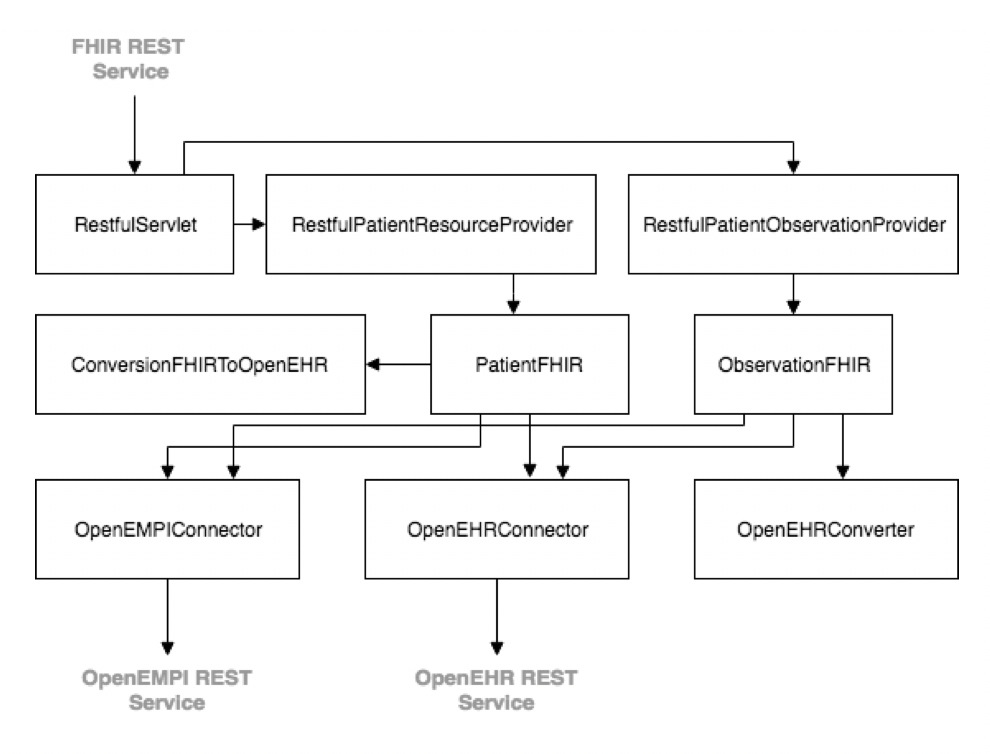
\includegraphics[width=0.8\columnwidth]{Figure1.png}
	\caption{NHS2 Architecture Layout} 
	\label{fig:oldarch}
\end{figure}

Whilst expressing a desire to improve the architecture of the existing system, the manner in which the system presented itself to external clients was essentially correct. It was important to retain the implementation of the FHIR protocol by using the HAPI FHIR framework and the exposition of OpenEHR and OpenEMPI data to FHIR clients, as well as the systems using the Unirest library, which facilitated communication with OpenEHR and OpenEHR systems through their respective REST APIs.

As a result of the time it took for the regression testing of the existing solution, it became apparent that a great deal of time was spent interrogating the JSON objects provided by calling the HAPI FHIR framework, as well as the EHR and EMPI REST services. To improve upon this, the Facade design pattern was used, isolating the complexity of interacting with the OpenEHR and OpenEMPI REST APIs behind a simple and easily tested facade, written in Java. Serialization was then used to convert the data returned by the REST APIs, JSON, and XML objects into Java objects. This facilitated easier interaction between the various services, as well as improved code reuse and encapsulation of REST API knowledge.

In between the FHIR and OpenEHR REST services, the routes of communication in the original system were replaced with an architecture based on the command pattern. Each FHIR operation that was supported; ‘read patient,’ for example, was represented as an object containing all the information needed to carry it out. Each operation was paired with one or more Executor classes, or classes containing the behaviour required to carry out the operation. A one to many relationship existed as the FHIR API supports both options on explicit targets (patients with a certain identifier, for example) or conditional targets where given search criteria are used to determine the target of the operation. The behaviour of explicit and condition operations can vary dramatically, therefore these were separated into different classes.

\begin{figure}[!!h] 
	\centering 
	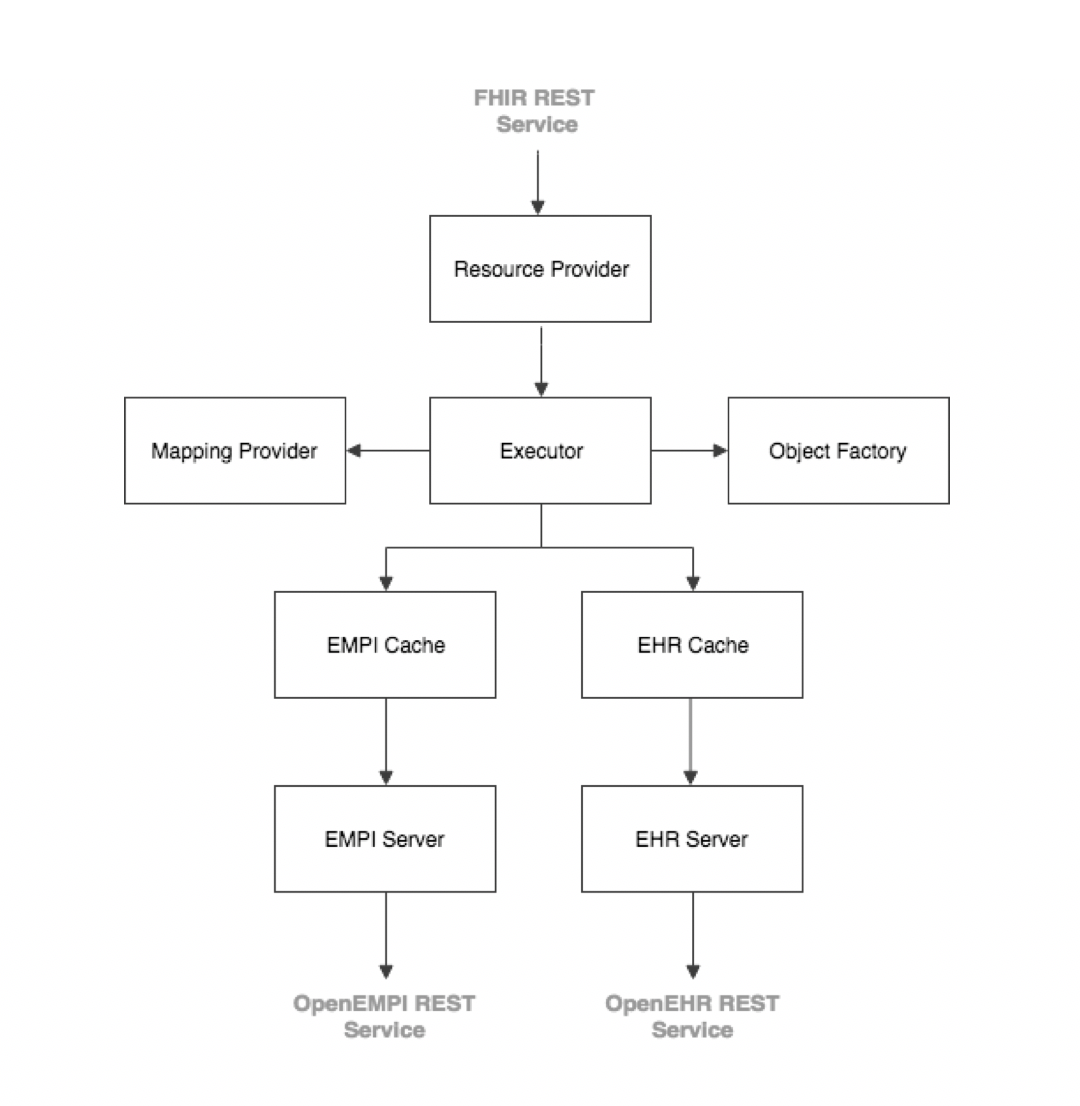
\includegraphics[width=0.8\columnwidth]{Figure2.png}
	\caption{New Architecture Layout} 
	\label{fig:new arch}
\end{figure}

The type conversion system is perhaps the central pillar of the OpenEHR Facade, converting data from FHIR requests into OpenEMPI and OpenEHR requests. To support the functionality required by the client, the conversion system needed to be improved in order to handle conversions involving both Patient and Observation data, as well as to handle type conversions specified in configuration provided by the user.

Converting between FHIR Patient and OpenEMPI Person data types was a relatively straightforward process, as both types contain roughly the same fields, although FHIR has less properties than OpenEMPI. The current solution implements most, but not all, patient properties, most notably contact information and address. These were not necessary to achieve the client’s objectives and, as such, were not attributed a high priority. Implementing these in the future would be a relatively straightforward process.

Converting between observations and medical data stored in the OpenEHR system was a much more complicated proposition. The fact that FHIR observations are requested by specifying a series of LOINC codes (snippet 1), six-digit numeric codes that uniquely identify a single medical attribute for a patient, constituted a core problem. For example, body mass index has the LOINC code 39156-5. On the other hand, to request medical data from an OpenEHR system, an AQL query (snippet 2), which is a structured natural language like query similar to SQL, must be provided. Once an AQL query is made, the results are returned as a set of name value pairs, which then need to be converted into a FHIR observation before being returned to the FHIR client who made the original request. 

\begin{figure}[!!h] 
	\centering 
	\includegraphics[width=0.8\columnwidth]{figure3.png}

\end{figure}

To implement the observation conversion process, a hybrid of the factory pattern with the adapter design patterns was used. Type conversions took place in a series of factory classes, each tasked with constructing a particular object, given another. Type conversion and communication with the OpenEHR service was coordinated by a mapping provider, either for basic mappings or for more advanced mappings, that is scripted mappings.

In their work, the previous team provided a proof of concept as to how users could specify the mapping between LOINC codes and AQL queries by providing only a select set of essential information. This forms the basis of the basic mapping. For each LOINC code, the user specifies the path to the value and its unit, along with the archetype identifier being queried. The system then handles the rest, using the information to construct an AQL query, execute it, and convert the result into a FHIR Observation. Snippet 3 shows an example of a basic mapping. 

\begin{figure}[!!h] 
	\centering 
	\includegraphics[width=0.8\columnwidth]{figure4.png}
\end{figure}

While basic mappings handle most type conversions, some mappings are more complicated and their needs couldn't be anticipated. To cope with this situation, a more advanced mapping type that allows users to provide a script was created, written in Javascript. This mapping performed the same actions as in the basic mapping, generating an AQL query for a given LOINC code and converting the results of executing the query into a FHIR observation. The script was executed at runtime, providing the user the full ability to modify the mapping process as they see fit. The script was executed using the Nashorn script engine built into Java and included protection for the insecurities inherent in executing user provided script.

\subsection{Performance Optimization}
To optimize the performance of the system, caching was introduced between the OpenEHR Facades communication with the OpenEHR and OpenEHR services. The caching solution was implemented using the proxy design pattern. Communication with external services, such as the OpenEHR service, was first abstracted behind an interface. A proxy version of this interface was then created, which delegated method calls onto the original concrete external service class. The results of this delegation were then cached for use with subsequent service calls with identical parameters. 

The dependency injection pattern, which had been used throughout the solution, was used to replace references to the original server implementation wherever it was used with the new cache proxy, by binding instances of the external services interface to the cache proxy implementation. 

The caching facility itself was handled by Caffeine, an open source but widely caching library, based on the Google Guava caching library. This allowed us to leverage a tried and tested caching implementation and to make use of a number of its cache maintenance features, providing the solution the ability to set the maximum number and expiry time of items in the cache. These settings were later added to our configuration user interface, allowing system administrators to configure the system as it suits them best.

\subsection{Network}
As alluded to in previous sections, the use of network services, notably the OpenEHR and OpenEMPI services, were refactored into classes representing each network service. This was done in order to lower coupling and promote code reuse. The new network service modules consist of a series of classes based on the REST architecture, handling sending REST requests and receiving REST responses. The module also provides significant improvements to authentication, including reauthentication on session token expiry and improvements to the network systems exception handling capability. Exceptions are also now produced for a greater number of situations, such as unexpected http statuses, expected resources being missing, and authentication failures. 

\subsection{User Configuration}
In the previous groups, solution mapping rules were hard coded, which was one of the reasons behind this system not being extensible. To resolve this problem, mapping rules were made configurable. A new configuration module was designed for handling the configuring requests. This module loads the content of configuration files stored in disk and provides reading, writing, and deleting services to the other parts of the system. 

To make the configuration functions easy to use, a Graphical User Interface (GUI) was also designed. With the help of Spring MVC, a framework to construct Java web-based programs that follows the Model View Controller pattern, the GUI was implemented as a set of webpages. This GUI supports two types of mapping configuring operations: Basic and Scripted (advanced). 

The Basic mode supports operations to mapping configurations that refer to data types, sharing a similar format. In this mode, users will be prompted to provide the values of several predefined attributes and the queries required for getting the target observations will be automatically generated.

However, some data types required by Growth Chart App present a more complicated format. They may have different number of attributes and the types of these attributes may vary. Additionally, the values of the attributes sometimes require further computation before they can be used. For these data types, the queries cannot be automatically generated. A Scripted mode was designed to support the manual specification by implementing a set of JavaScript functions. 


\begin{figure}[!!h] 
	\centering 
	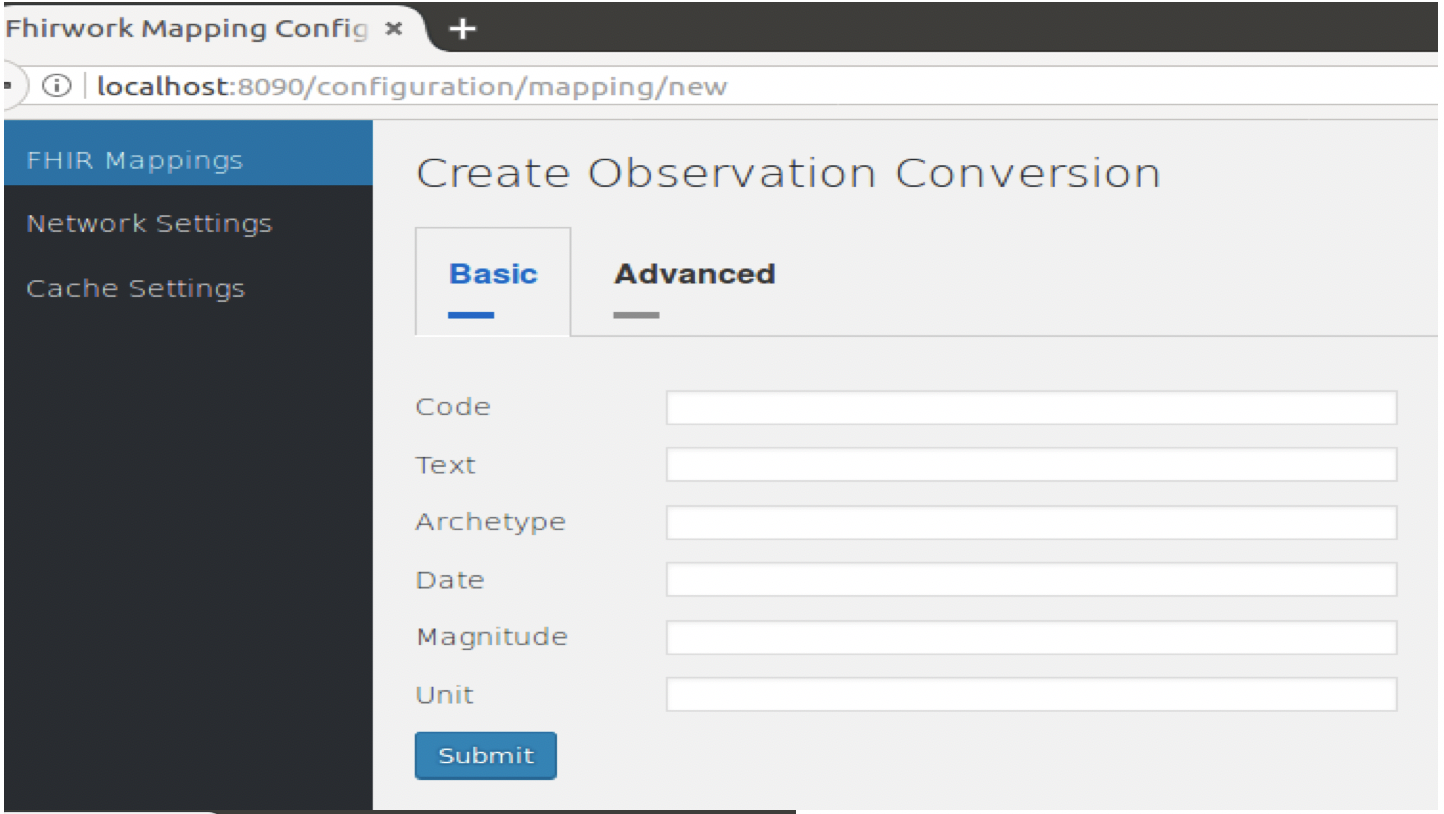
\includegraphics[width=0.8\columnwidth]{basicmapping.png}
	\caption{Basic Mapping Mode	} 
	\label{fig:basicmap}
\end{figure}

\begin{figure}[!!h] 
	\centering 
	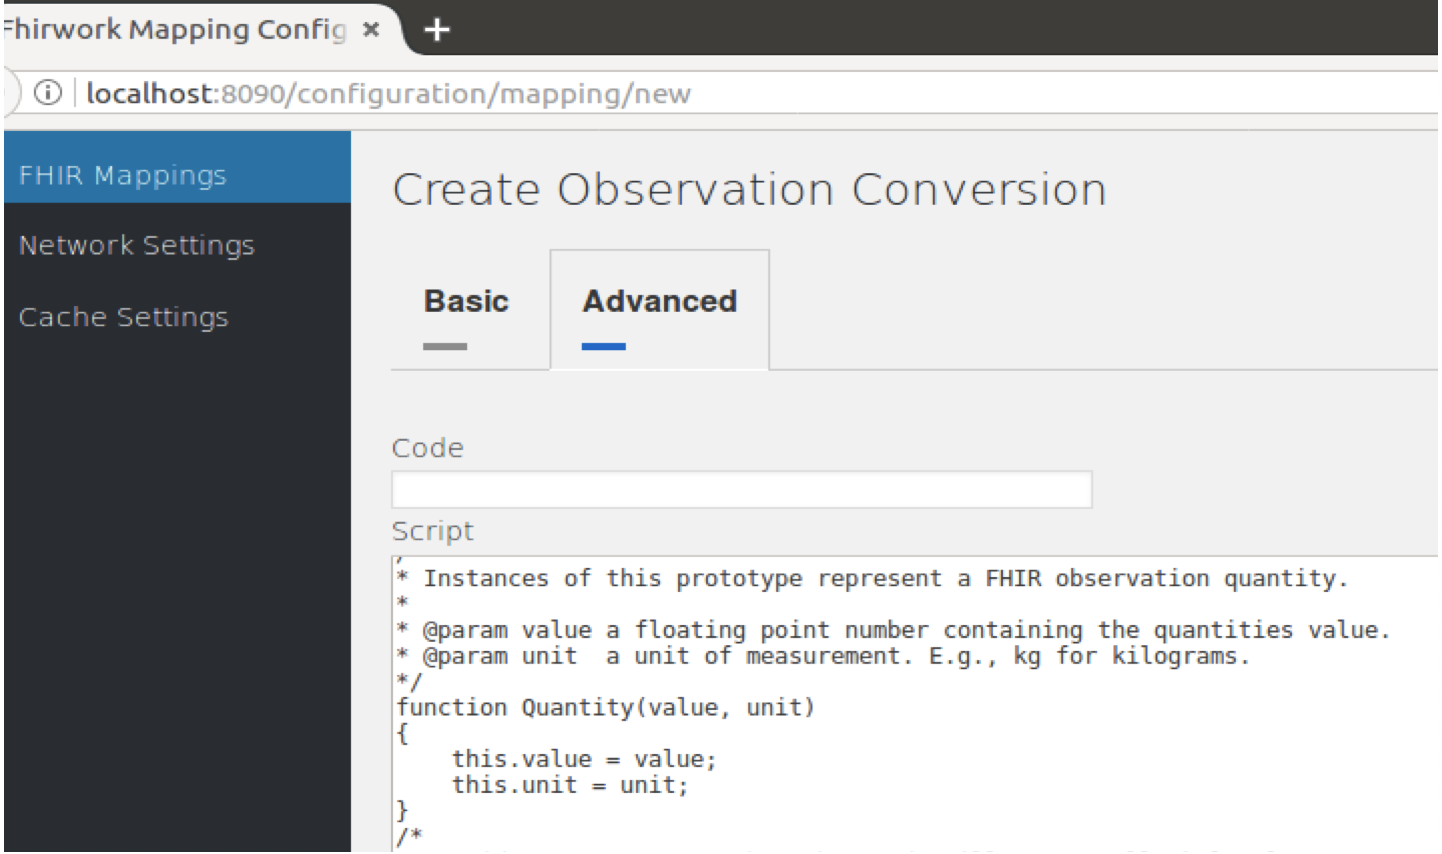
\includegraphics[width=0.8\columnwidth]{advancedmapping.png}
	\caption{Advanced (Scripted) Mapping ModeI} 
	\label{fig:advancedmap}
\end{figure}

Aside from handling mapping configurations, the module was extended to manage different types of configurations, for example, network configurations. The modification to network configurations is also supported in the GUI. 

As part of the client’s objective of improving the performance of the system, caching was enabled to optimise performance. The configuration GUI also provides configurability for this feature. It allows the user to decide whether caching should be enabled. Additionally, the parameters about how much information should be cached and how long the cached information could be retained can also be specified.

\begin{figure}[!!h] 
	\centering 
	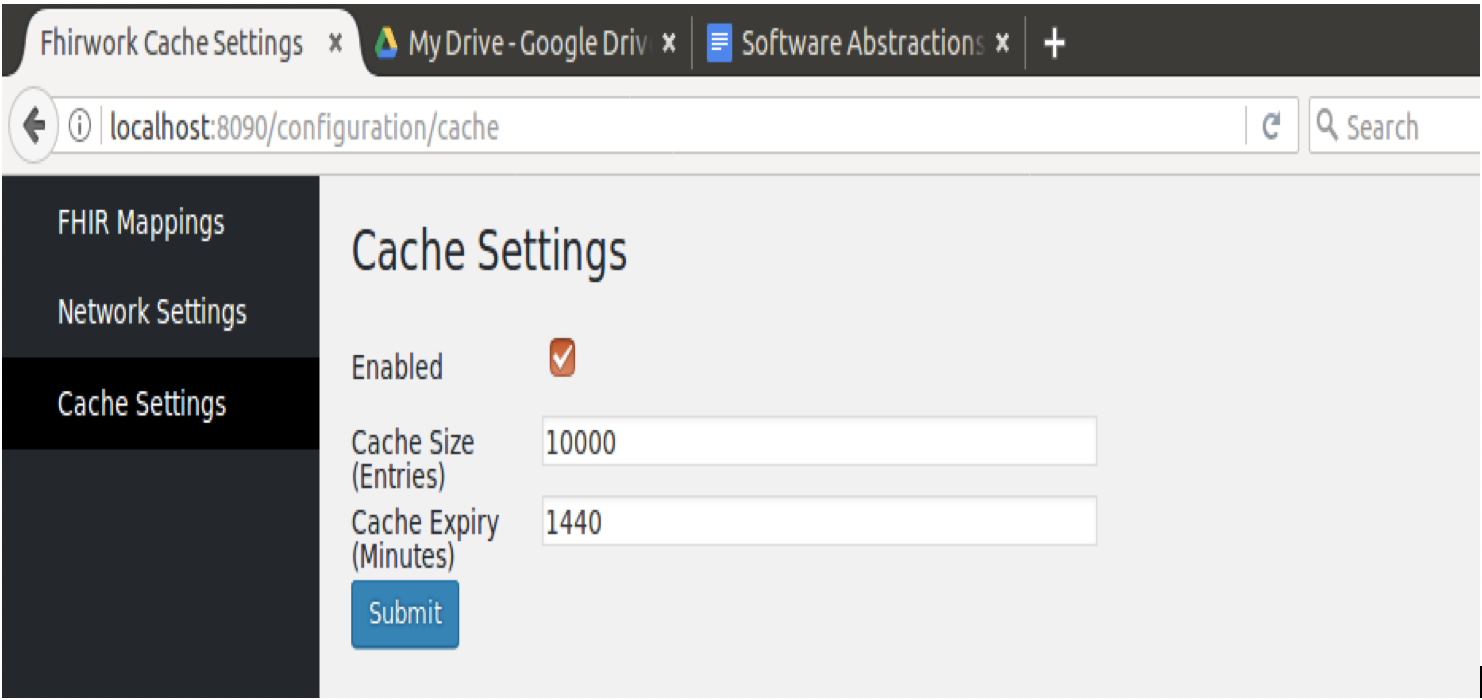
\includegraphics[width=0.8\columnwidth]{caching.png}
	\caption{Caching GUI} 
	\label{fig:cache}
\end{figure}

\subsection{Bonfhir Manual Testing Tool}
The Bonfhir manual testing tool is a node.js web application that provides a medium to visually test whether the implementations of the HAPI-FHIR api operations and their mappings to EHR and OPEN-EMPI operations are correct. It also takes a minimalistic approach and only has four relevant pages/operations: 
\begin{itemize}
\item The “patients” page allows the user to view all the patients currently stored in the FHIR server database. When a user views this page, the application uses the HAPI-FHIR implementation to make an HTTP GET request for all patients in the database. The implementation generates a response by making the appropriate requests for required data fields to the EMPI server.
\item In the “patients” section, it is possible for the user to add a patient. When this feature is used, the application makes an HTTP POST request to the HAPI-FHIR implementation which, in turn, parses the inputted data and stores the relevant fields in the EMPI server.
\item “View all observations currently stored for a patient.” When this feature is used, the application makes a HTTP GET request to the HAPI-FHIR implementation for all observations for a certain patient. The implementation generates a response by making the appropriate requests for required data fields to the OpenEHR and EMPI servers and mapping them back into a FHIR JSON object, which the Bonfhir application then consumes and presents in a table format.
\item “Launch the growth chart app for a specific patient.” This feature demonstrates that the application fully supports the growth chart.
\end{itemize}

\section{Evaluation, Testing, Performance} 
The developments made this year in comparison to the previous year include many non-functional improvements as well. Continuous integration was implemented with Travis CI so that the changes made to the solution were automatically built and tested. Strict standards for code quality and style checking were set. If the new code violates the criterias, the build is considered broken. When checked with the Codacy tool and java checkstyle, the project’s score more than doubled from last year’s 47% to 99%. Both unit testing and integration testing were set up so that they would run against every code change in order to ensure no regressions were introduced. This resulted in an improved code coverage of 78% compared to last year’s 58% (or lower than 30% when external dependencies are accounted for). Manual testing can now also be done with the Bonfhir tool, which has the advantage of allowing for live product demonstrations.

\begin{figure}[!!h] 
	\centering 
	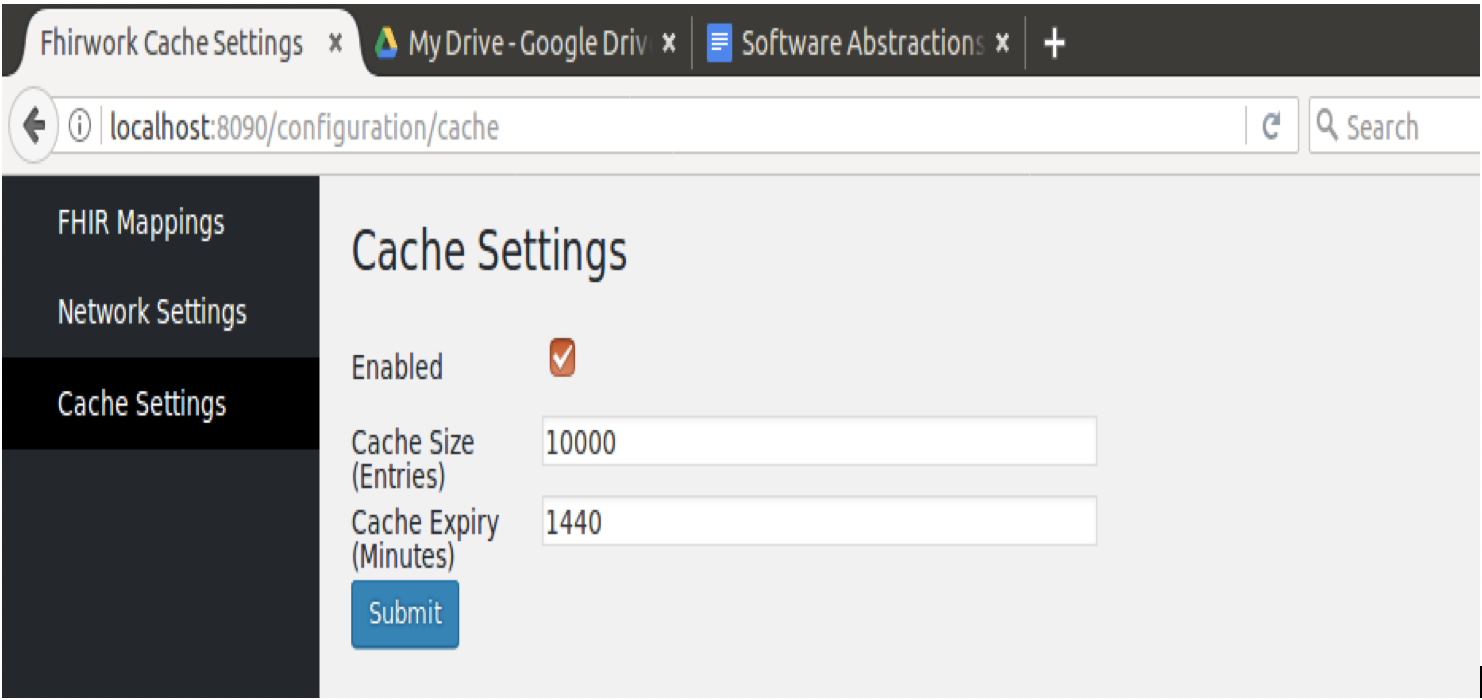
\includegraphics[width=0.8\columnwidth]{caching.png}
	\caption{Performance Testing Results (1000 concurrent users)} 
	\label{fig:performance}
\end{figure}

The product’s performance was tested with JMETER, taking into account the two main operations; get patient and get observation. Under the same load, the average response time for the get patient query was 18% faster and the average response time for the get observation query was 508% faster. The improvements were mainly due to the implementation of caching. Caching allows for significant improvement in performance for this specific use because of how the Growth Chart application operates. When using the Growth Chart, a single patient and all observations for that patient are queried consecutively until the Growth Chart is viewed for a new patient. This allows the product to cache the current information being used and respond to the consecutive queries much faster. Effectively, this means that, while users may not experience improvements in speed when they first view a patient’s chart, the response time will be much faster when that user tweaks exactly which kind of data he or she would like to view for that patient, thus improving performance while the app is in use.

\section{Future Work} 

In the future, it is possible to enlarge the scope of this project by supporting more of the FHIR protocol, effectively enabling the usage of more charts. This can be easily done because of the current modular design. The multitude of resource providers and executors all use the same structure. It is therefore easy to extend and specialize their functionalities.

Furthermore, it is also possible to improve the current implementation in order to productize the project. Even though the current version offers the possibility for a live demo and the final product meets the client’s requirements, it has not been tested enough to match industry standards. With some added exception, handling and scalability testing the current project can be made into an actual industry-ready product.

Finally, it is possible to take the current partial implementation of EHR and EMPI servers as Java Rest libraries and make them into their own projects. FHIR provides its own REST library called HAPI-FHIR, making it very easy to build technologies that depend on or interact with FHIR. However, EHR and EMPI don’t really provide a similar library.

\bibliographystyle{ACM-Reference-Format} \bibliography{bibliography}

\end{document}
